\documentclass[tikz,border=8pt]{standalone}
\usepackage{amsmath}
\usepackage{pgfplots}
\pgfplotsset{compat=1.18}
\usetikzlibrary{arrows.meta}
\begin{document}
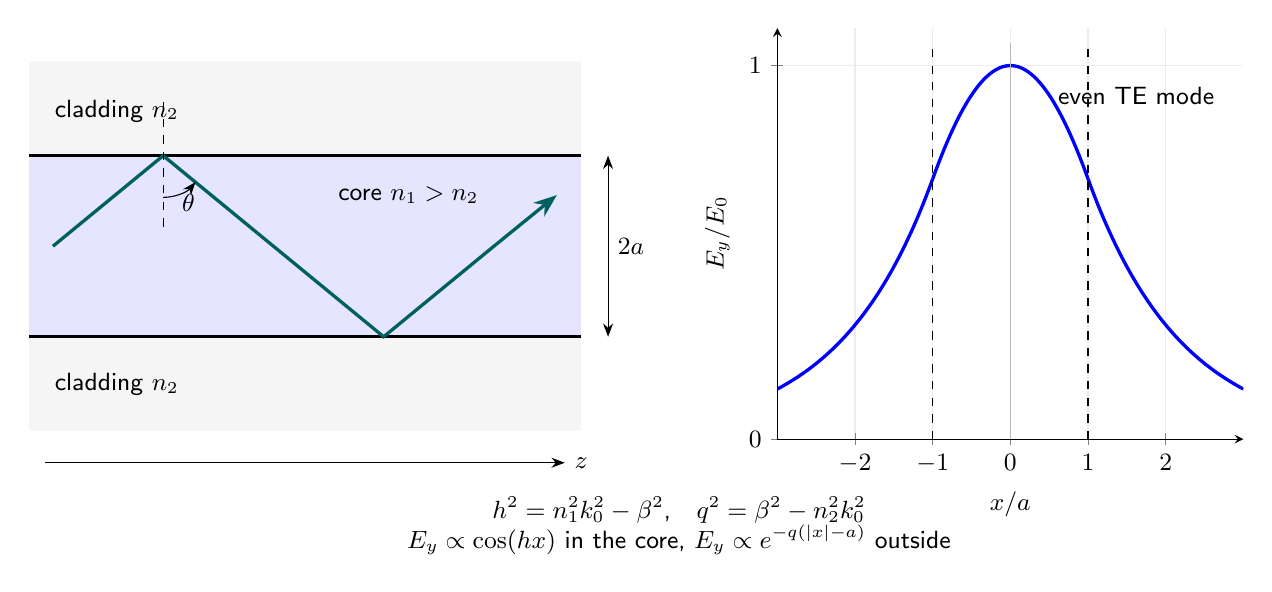
\begin{tikzpicture}[font=\sffamily\small,>=Stealth]
  \begin{scope}
    \fill[blue!10] (0,-1.15) rectangle (7,1.15);
    \fill[gray!8] (0,1.15) rectangle (7,2.35);
    \fill[gray!8] (0,-2.35) rectangle (7,-1.15);
    \draw[very thick] (0,1.15)--(7,1.15) (0,-1.15)--(7,-1.15);
    \draw[->,teal!75!black,very thick]
      (.3,0)--(1.7,1.15)--(3.1,0)--(4.5,-1.15)--(5.9,0)--(6.7,.65);
    \draw[dashed] (1.7,.25)--(1.7,1.9);
    \draw[->] (1.7,.62) arc[start angle=-90,end angle=-39.4,radius=.53];
    \node at (2.02,.55) {$\theta$};
    \node[anchor=west] at (.2,1.72) {cladding $n_2$};
    \node[anchor=west] at (3.8,.65) {core $n_1>n_2$};
    \node[anchor=west] at (.2,-1.75) {cladding $n_2$};
    \draw[<->] (7.35,-1.15)--(7.35,1.15) node[midway,right] {$2a$};
    \draw[->] (.2,-2.75)--(6.8,-2.75) node[right] {$z$};
  \end{scope}
  \begin{scope}[xshift=9.5cm,yshift=-2.45cm]
  \pgfmathsetmacro{\uval}{0.8}
  \pgfmathsetmacro{\wval}{\uval*tan(deg(\uval))}
  \begin{axis}[
    width=7.5cm,height=6.8cm,
    axis lines=left,xmin=-3,xmax=3,ymin=0,ymax=1.1,
    xlabel={$x/a$},ylabel={$E_y/E_0$},
    xtick={-2,-1,0,1,2},ytick={0,1},
    grid=both,grid style={gray!15}]
    \addplot[blue,very thick,domain=-3:-1,samples=80]
      {cos(deg(\uval))*exp(\wval*(x+1))};
    \addplot[blue,very thick,domain=-1:1,samples=100]
      {cos(deg(\uval*x))};
    \addplot[blue,very thick,domain=1:3,samples=80]
      {cos(deg(\uval))*exp(-\wval*(x-1))};
    \draw[dashed] (axis cs:-1,0)--(axis cs:-1,1.05);
    \draw[dashed] (axis cs:1,0)--(axis cs:1,1.05);
    \draw[gray!55] (axis cs:0,0)--(axis cs:0,1.06);
    \node[anchor=east] at (axis cs:2.75,.92) {even TE mode};
  \end{axis}
  \end{scope}
  \node[align=center] at (8.25,-3.55)
    {$h^2=n_1^2k_0^2-\beta^2$,\quad $q^2=\beta^2-n_2^2k_0^2$\\
     $E_y\propto\cos(hx)$ in the core, $E_y\propto e^{-q(|x|-a)}$ outside};
\end{tikzpicture}
\end{document}
